



\begin{figure}[H]
    \centering	
    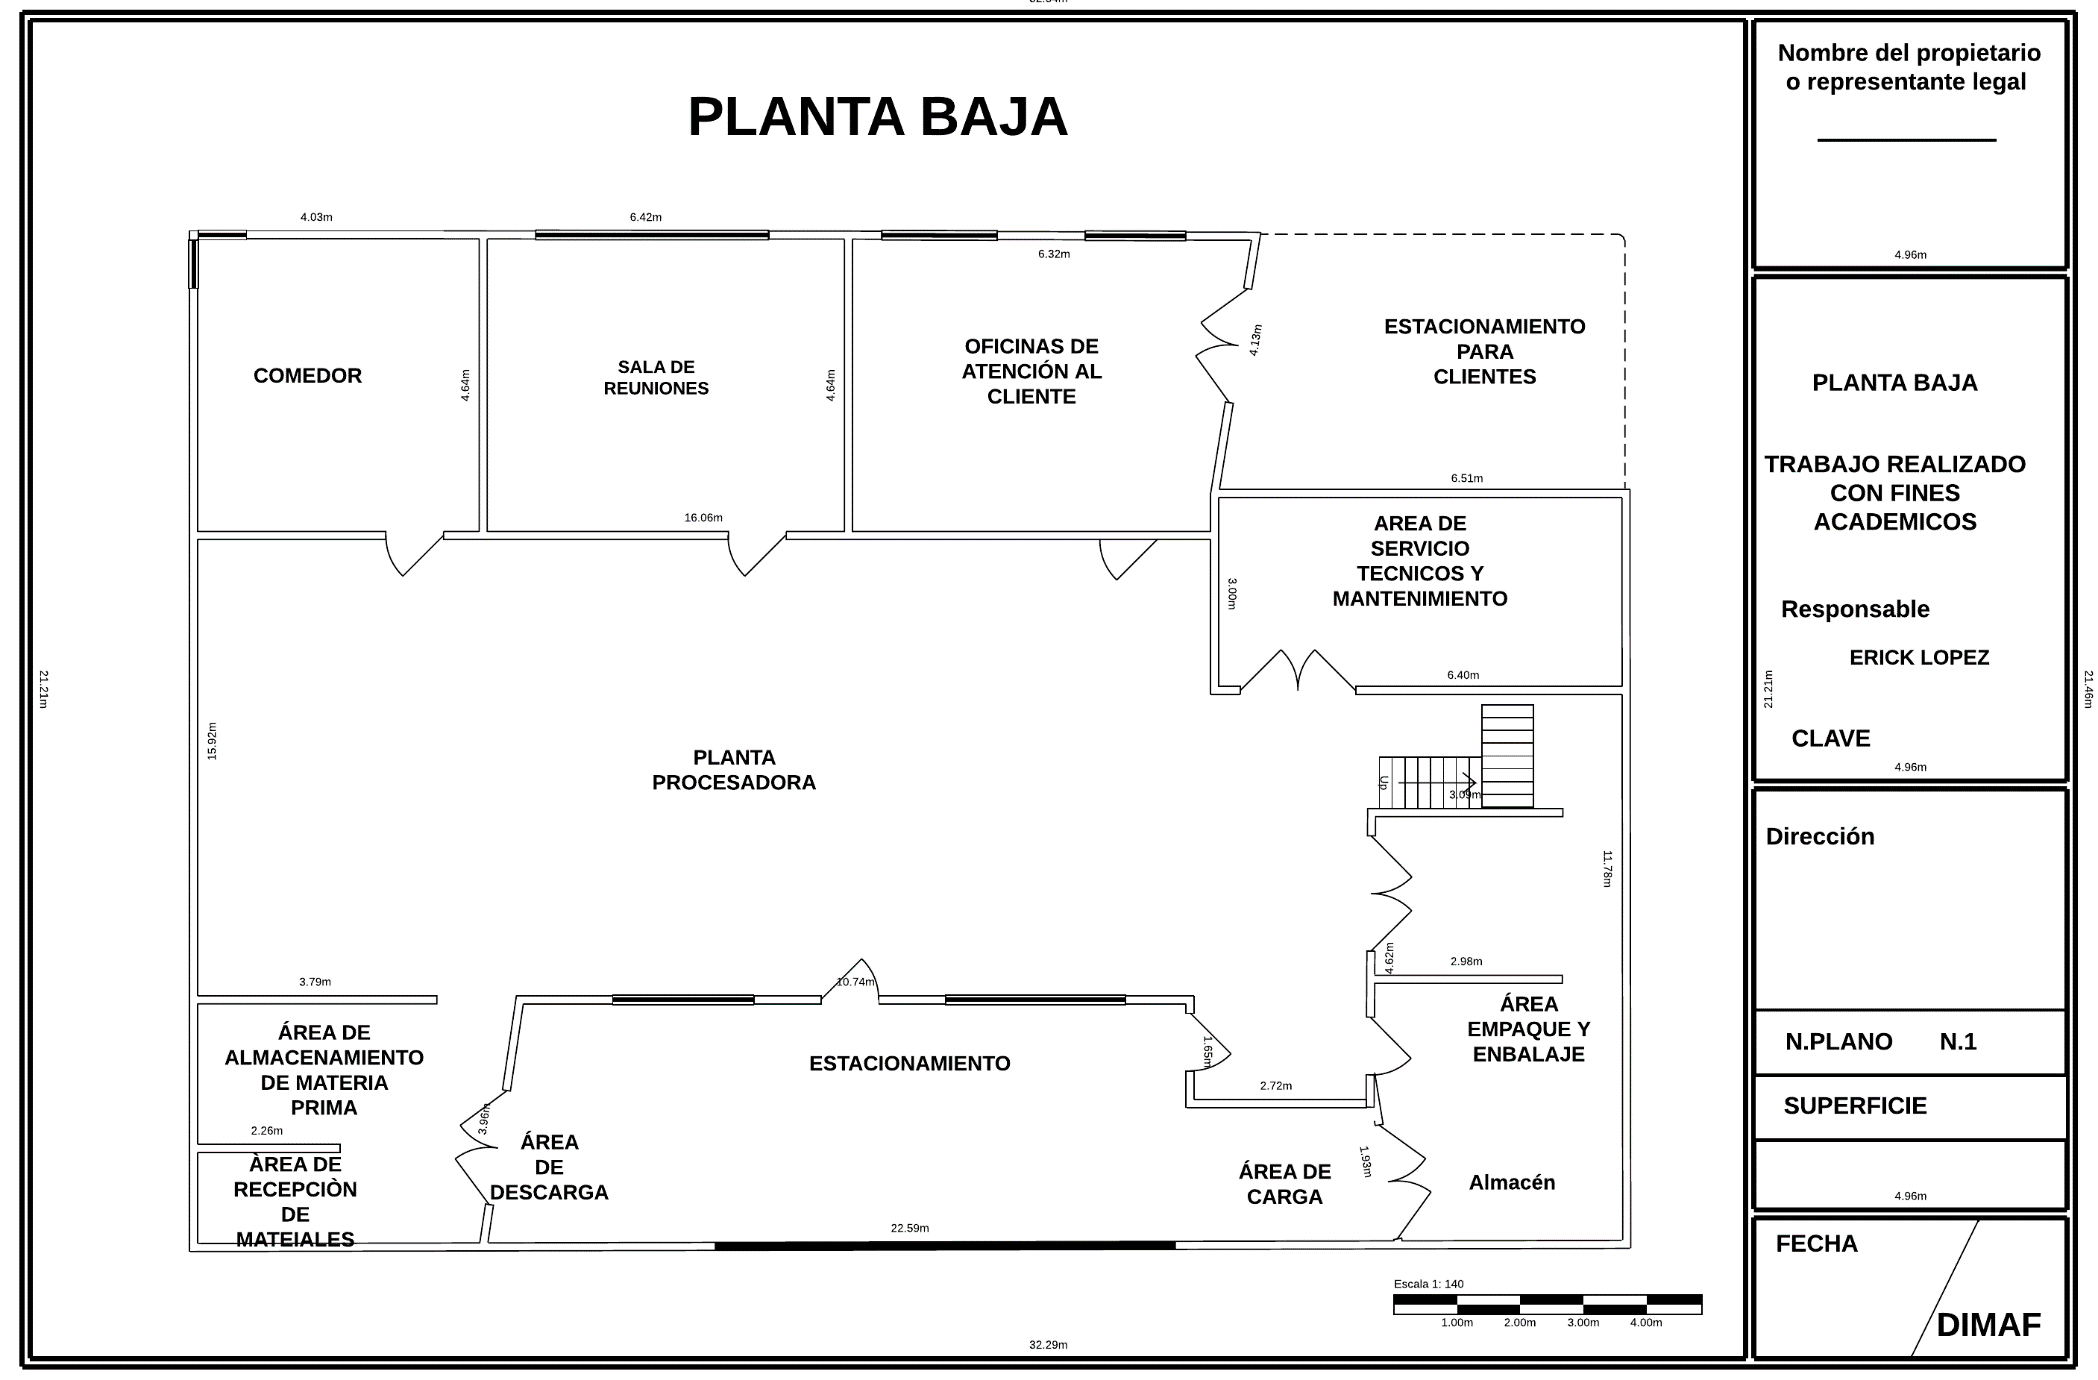
\includegraphics[angle=90,width=1.0\textwidth]{chapters/image1_.png} 
    \caption{Planta baja}
\label{fig:croquis190125}
\end{figure}

\begin{figure}[H]
    \centering	
    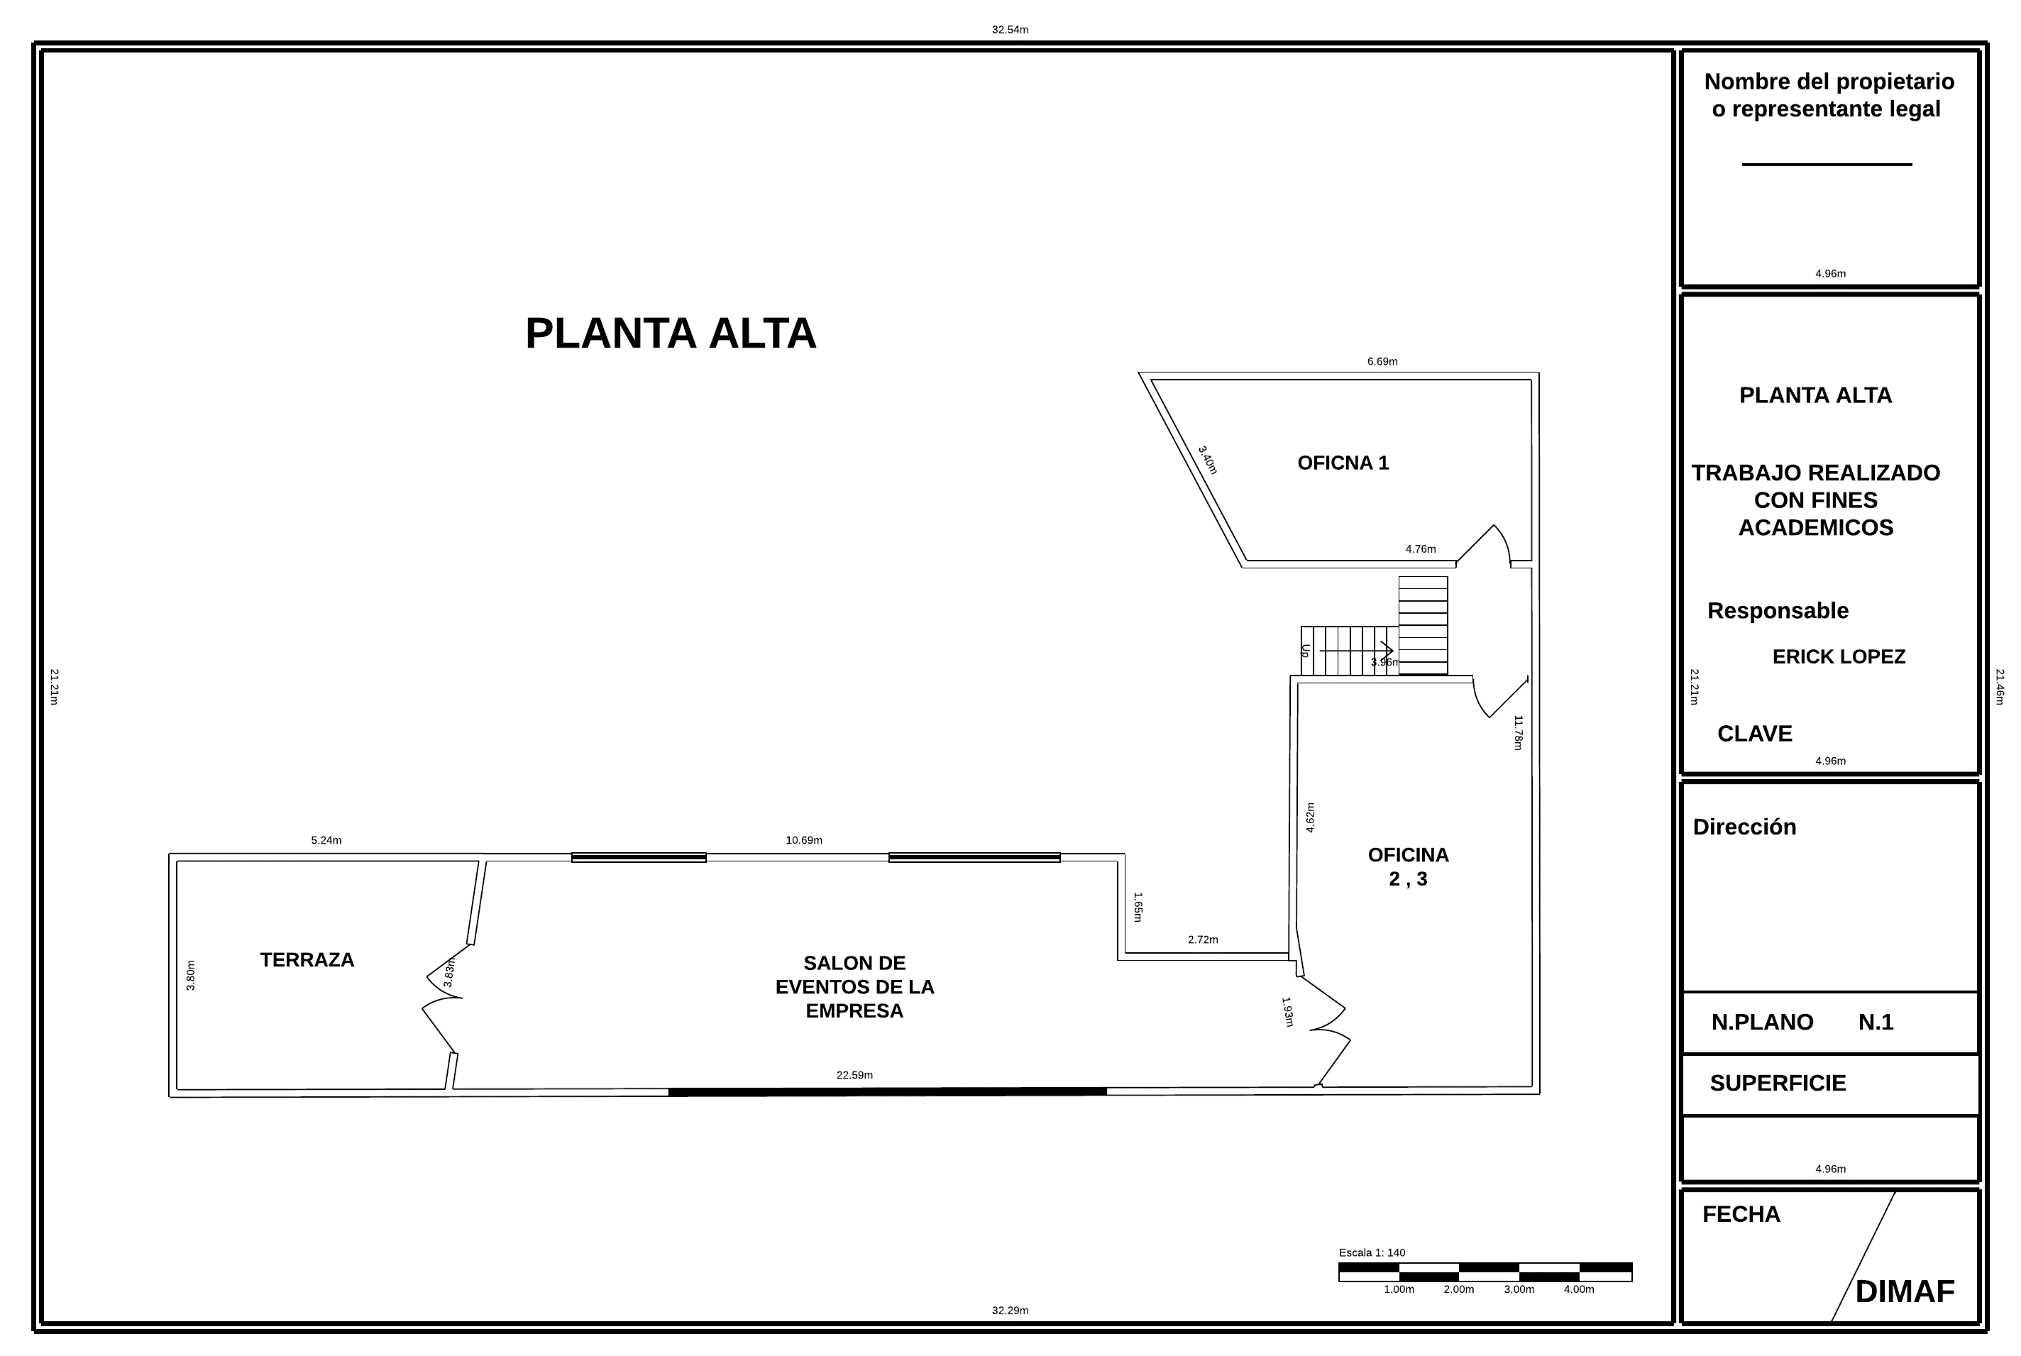
\includegraphics[angle=90,width=1.0\textwidth]{chapters/image2_.png} 
    \caption{Planta alta}
\label{fig:croquis190125}
\end{figure}

\begin{figure}[H]
    \centering	
    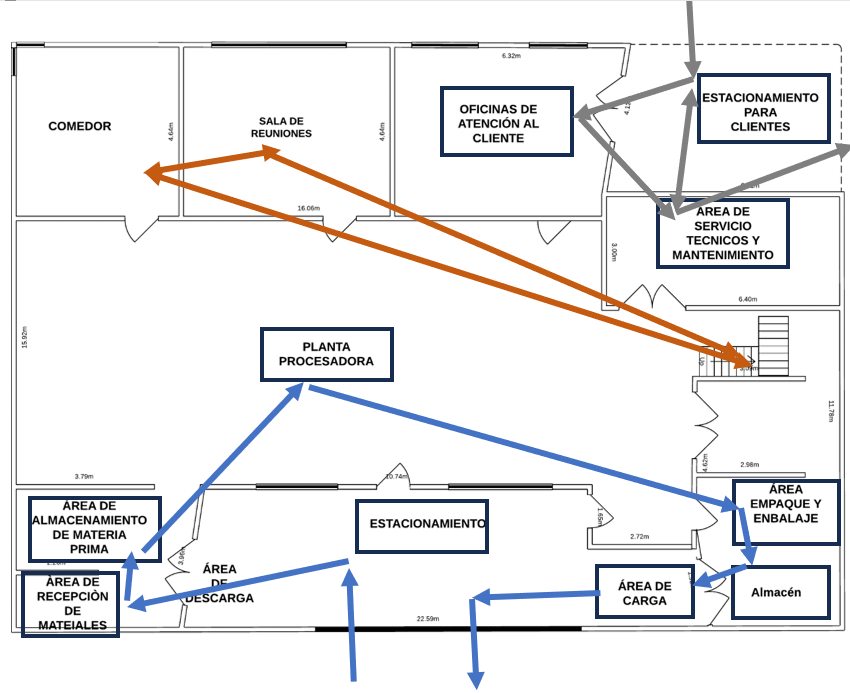
\includegraphics[angle=90,width=0.75\textwidth]{chapters/ELC_HILOS.png} 
    \caption{Diagrama de hilos}
\label{fig:croquis190125}
\end{figure}

Se tienen 3 principales hilos los cuales comprenden a 

1. Color gris

Es cuando una persona externa visita la empresa y esta desea un servicio técnico, atención a cliente o un acercamiento más a la empresa.

2. Color naranja

Área que recorre el personal administrativo y estos se conectan directamente a la segunda planta con las demás áreas administrativas.

3. Color azul 

Es la ruta que toman la contracción del producto desde recepción de materia prima hasta la entrega el producto final este camino es unidireccional, ya que no se puede regresar el material a un estado anterior. 

\begin{figure}[H]
    \centering	
    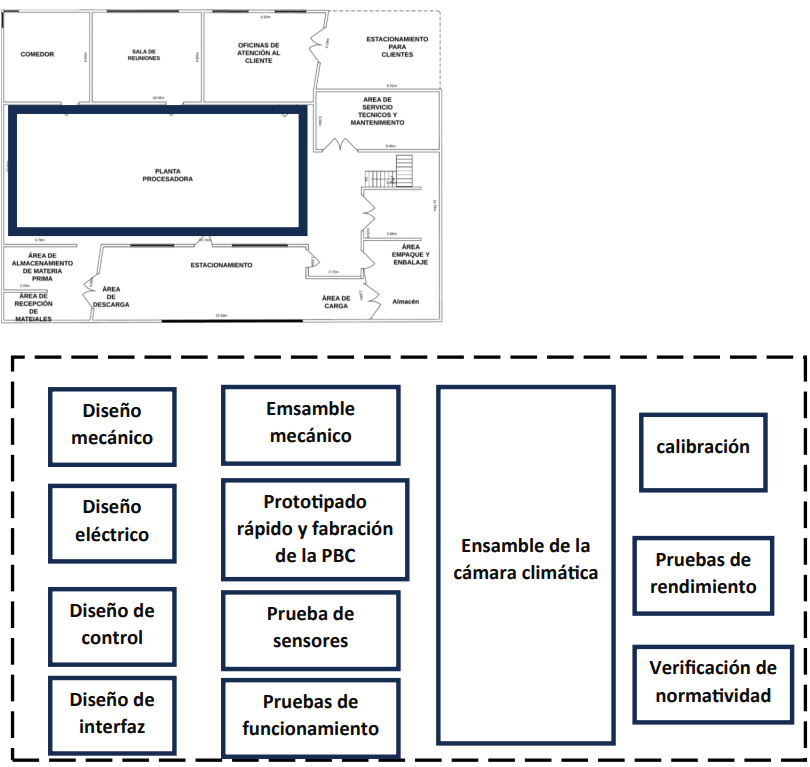
\includegraphics[angle=0,width=0.67\textwidth]{chapters/ELC_DIAGRAM.png} 
    \caption{Diagrama de distribución del área de producción}
\label{fig:croquis190125}
\end{figure}

Para poder producir las cámaras climáticas en necesario tener una distribución uniforme y las áreas no deben de estar alejadas, ya que nos reduce el tiempo de movimiento de materiales además de poder interactuar con las demás área para un correcto flujo y detección de errores.

\begin{figure}[H]
    \centering	
    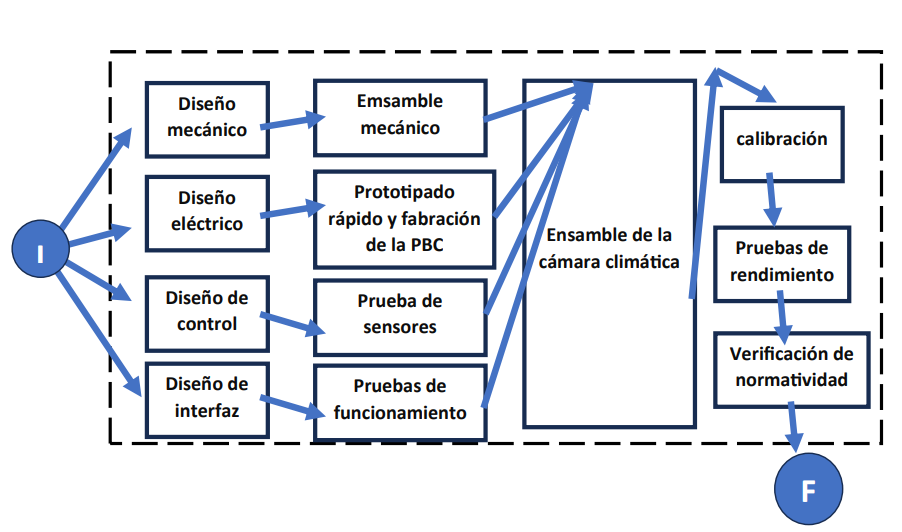
\includegraphics[angle=0,width=0.70\textwidth]{chapters/ELC_DIAGRAM2.png} 
    \caption{Diagrama hilos de la distribución del área de producción}
\label{fig:croquis190125}
\end{figure}

Se diseñó el área de producción para poder tener 4 áreas en este caso trabajando al mismo tiempo para aumentar efectividad y reducir los tiempos con ello podemos desarrollar productos más rápidos y permitir realizar productos personalizados cuando sea su caso. 
%----------------------------------------

